\subsection{Introducción.}
\begin{frame}
  \frametitle{Motivación.}
  Observemos el siguiente caso partícular de polígono simple:
  
  \begin{center} 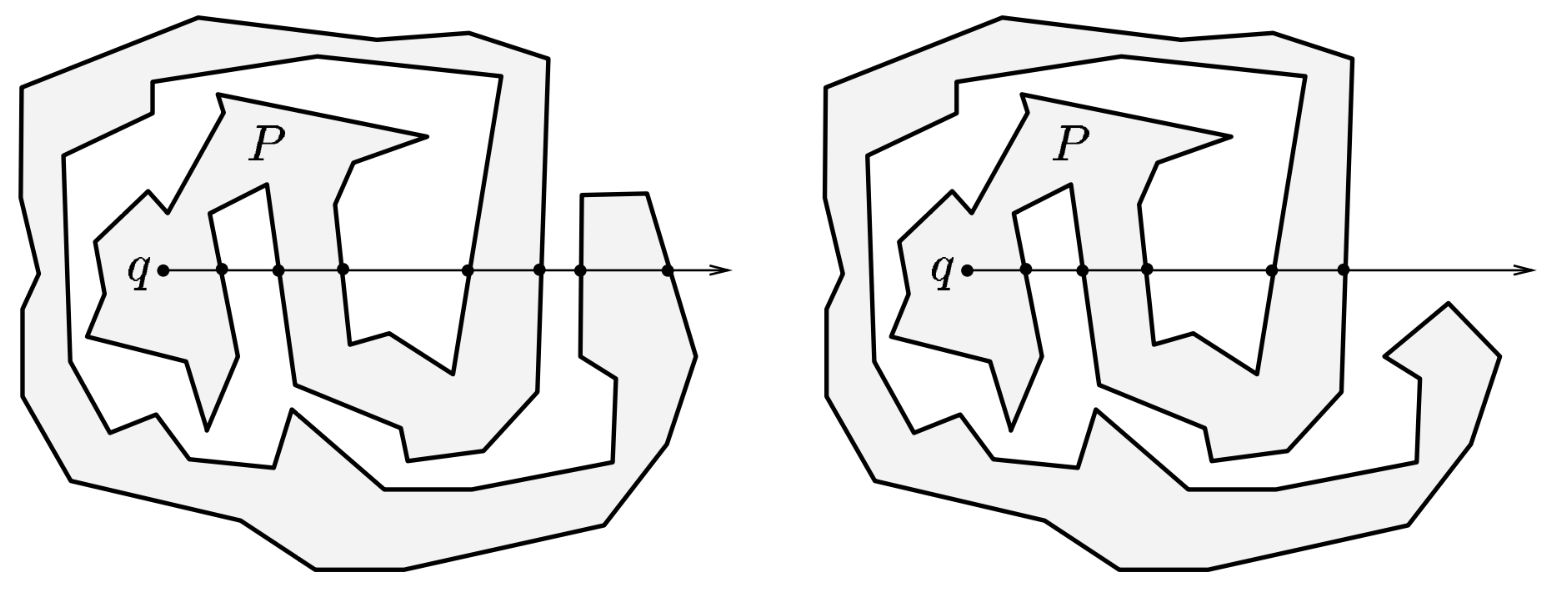
\includegraphics[width=0.55 \paperwidth]{images/Revoluciones.png} \end{center}

  El polígono de la izquierda tiene como número de revoluciones $2$ y el polígono
  de la derecha tiene cómo número de revoluciones $1$.
\end{frame}

\begin{frame}
  \frametitle{Poda de polígonos simples.}
  %\framesubtitle{Polígono de visibilidad.} %%Subtítulo de la diapositiva (opcional)
  Dado un polígono simple $P$ y un punto $q \in P$, calcular el polígono podado $P_1 \subseteq P$
  simple tal que $P_1$ contiene tanto a $V(q)$ como a $q$ y el número de revoluciones respecto de
  $q$ es a lo más $1$.  
\end{frame}

\subsection{Ejecución.}
% Estamos aquí ...
\begin{frame}
  \frametitle{Ejecución simple.}
  \centering 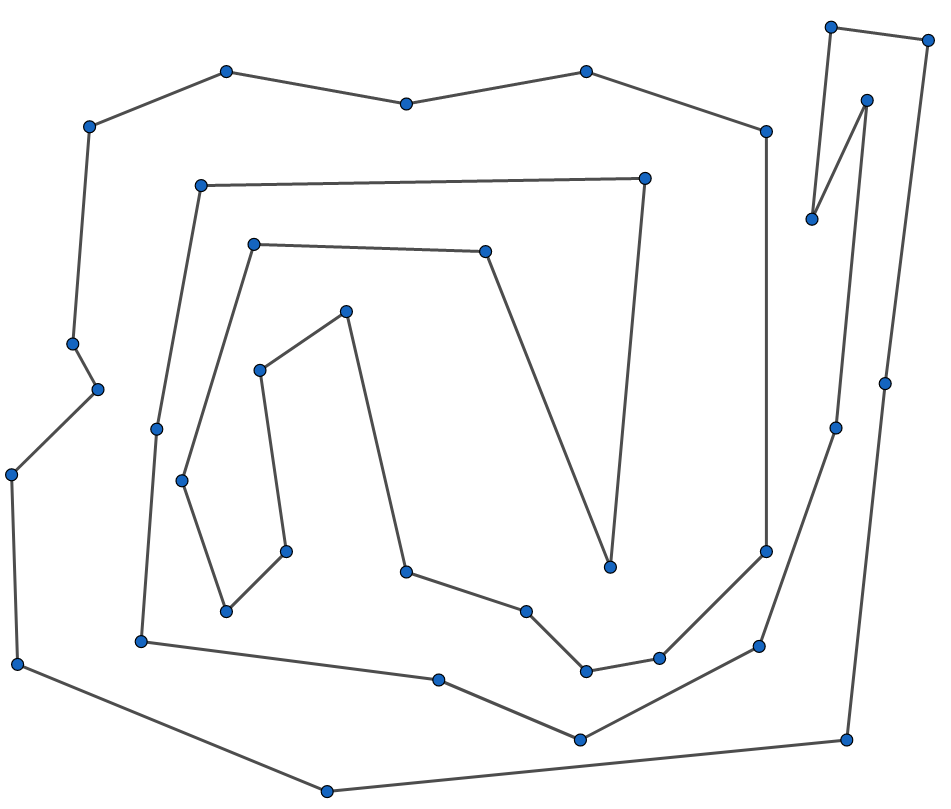
\includegraphics[width=0.45 \paperwidth]{images/Poda/1.png}
\end{frame}

\begin{frame}
  \centering 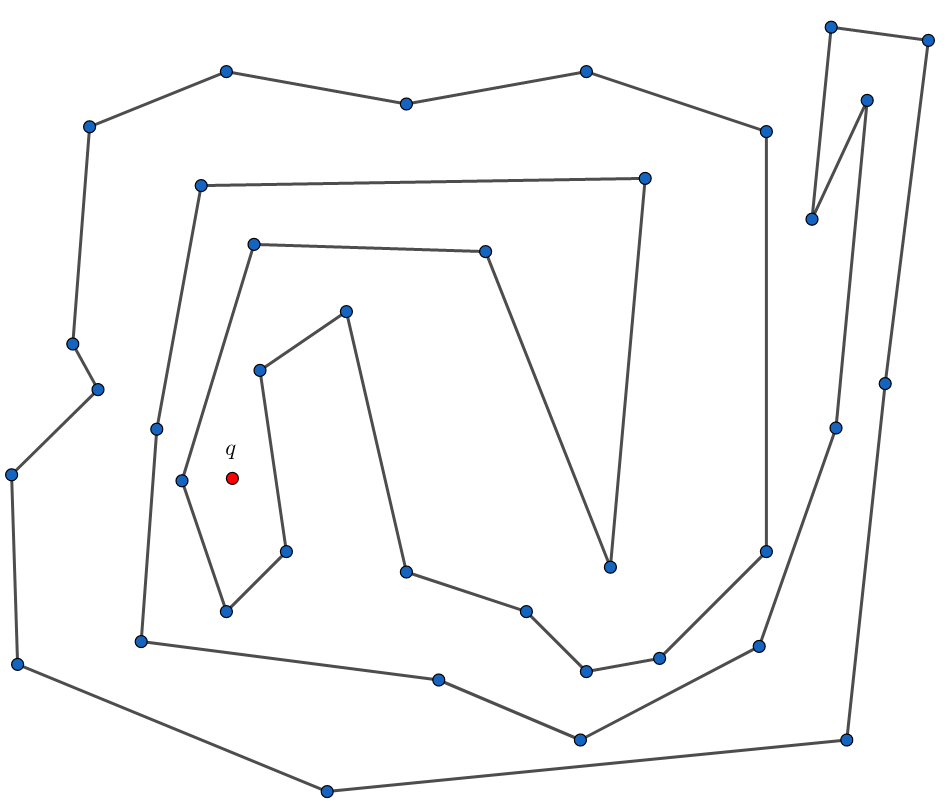
\includegraphics[width=0.45 \paperwidth]{images/Poda/2.png}
\end{frame}

\begin{frame}
  \centering 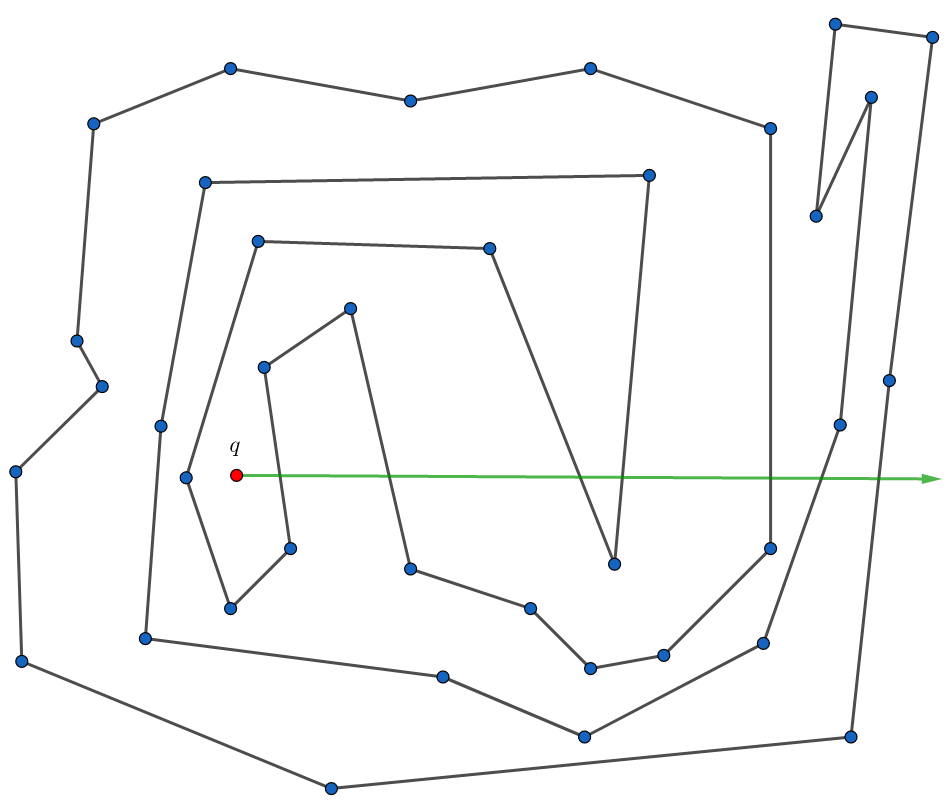
\includegraphics[width=0.45 \paperwidth]{images/Poda/3.png}
\end{frame}

\begin{frame}
  \centering 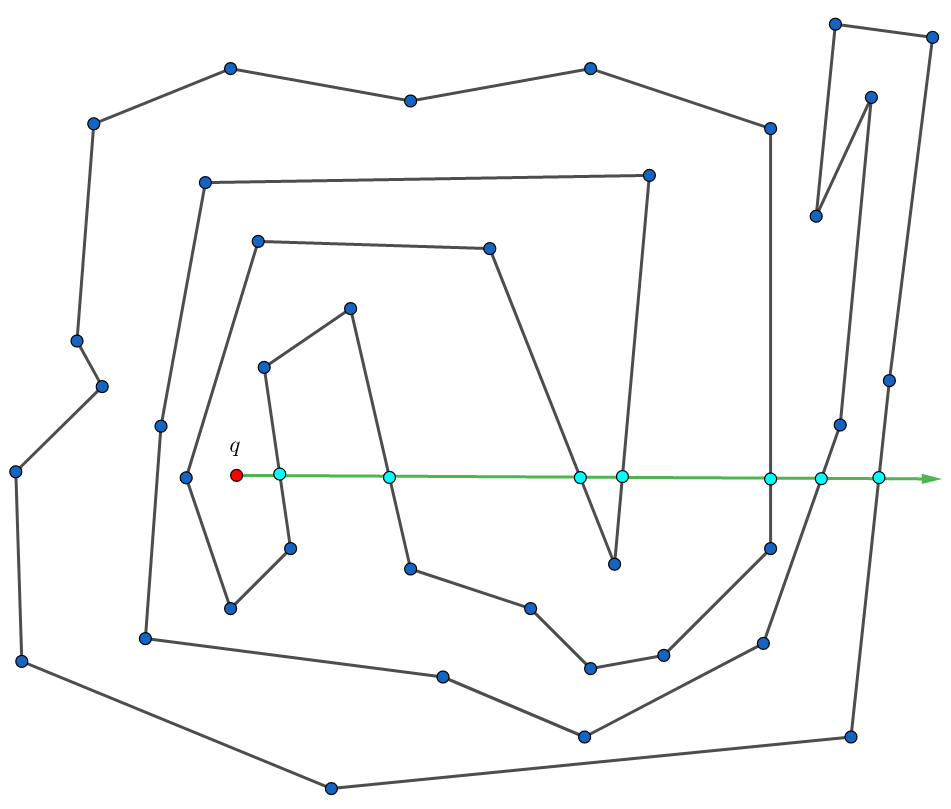
\includegraphics[width=0.45 \paperwidth]{images/Poda/4.png}
\end{frame}

\begin{frame}
  \centering 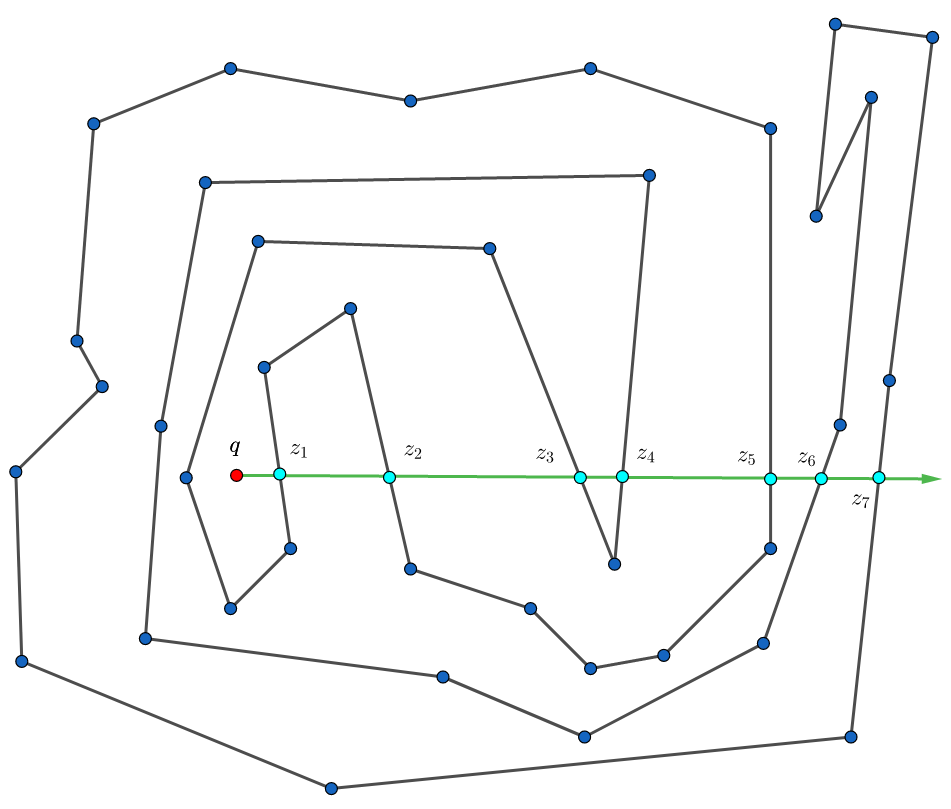
\includegraphics[width=0.45 \paperwidth]{images/Poda/5.png}
\end{frame}

\begin{frame}
  \centering 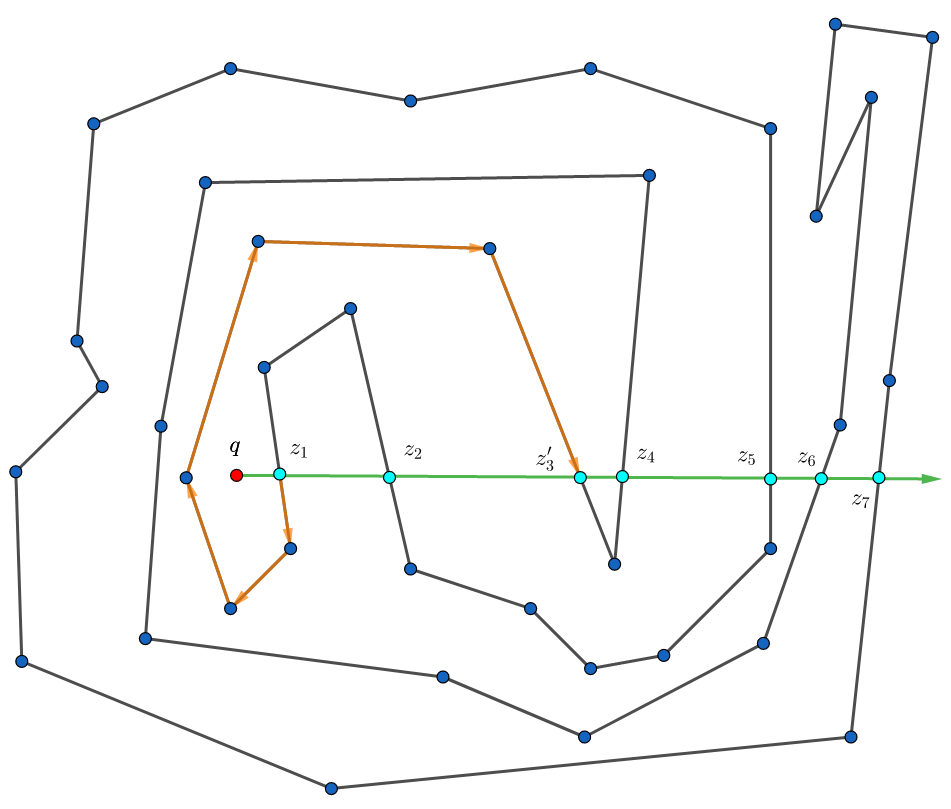
\includegraphics[width=0.45 \paperwidth]{images/Poda/6.png}
\end{frame}

\begin{frame}
  \centering 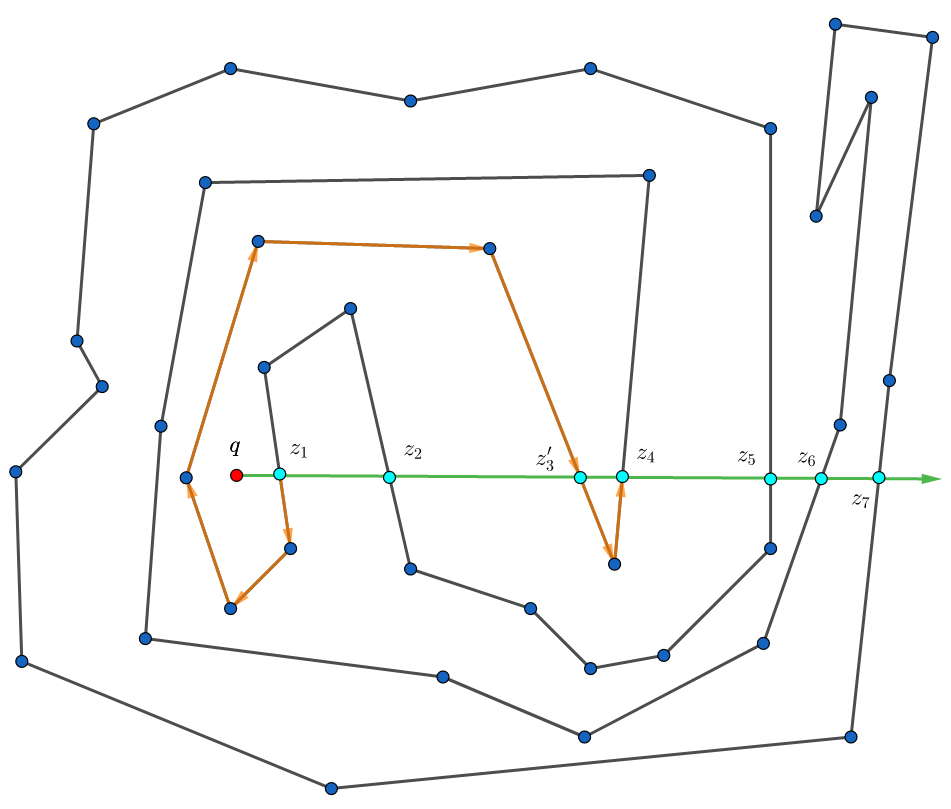
\includegraphics[width=0.45 \paperwidth]{images/Poda/7.png}
\end{frame}

\begin{frame}
  \centering 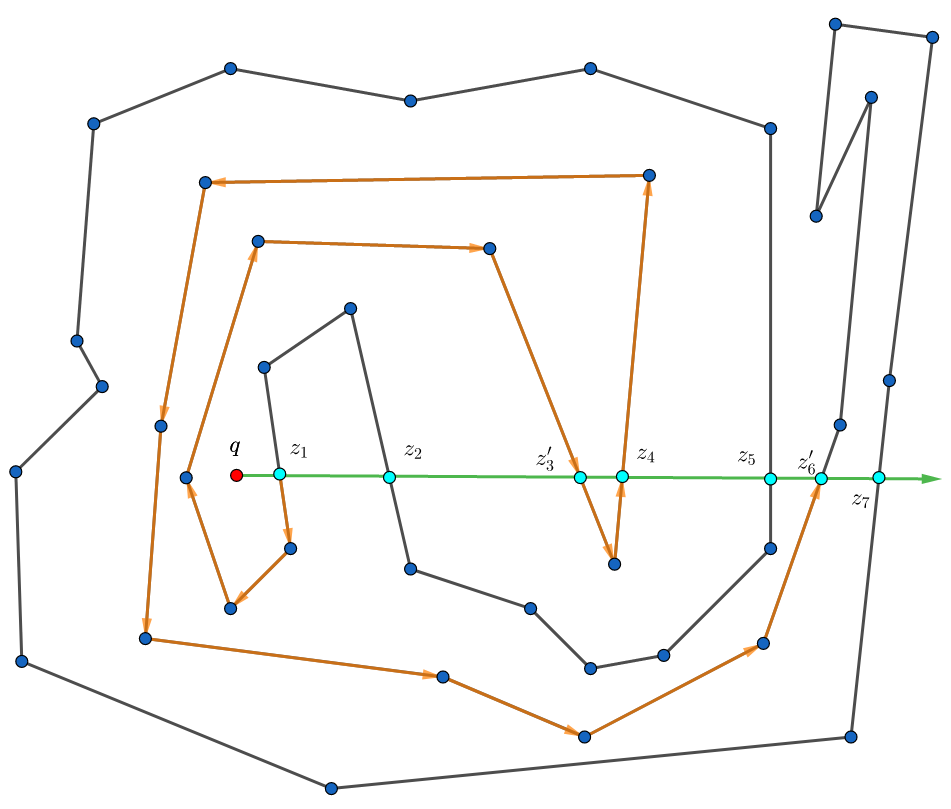
\includegraphics[width=0.45 \paperwidth]{images/Poda/8.png}
\end{frame}

\begin{frame}
  \centering 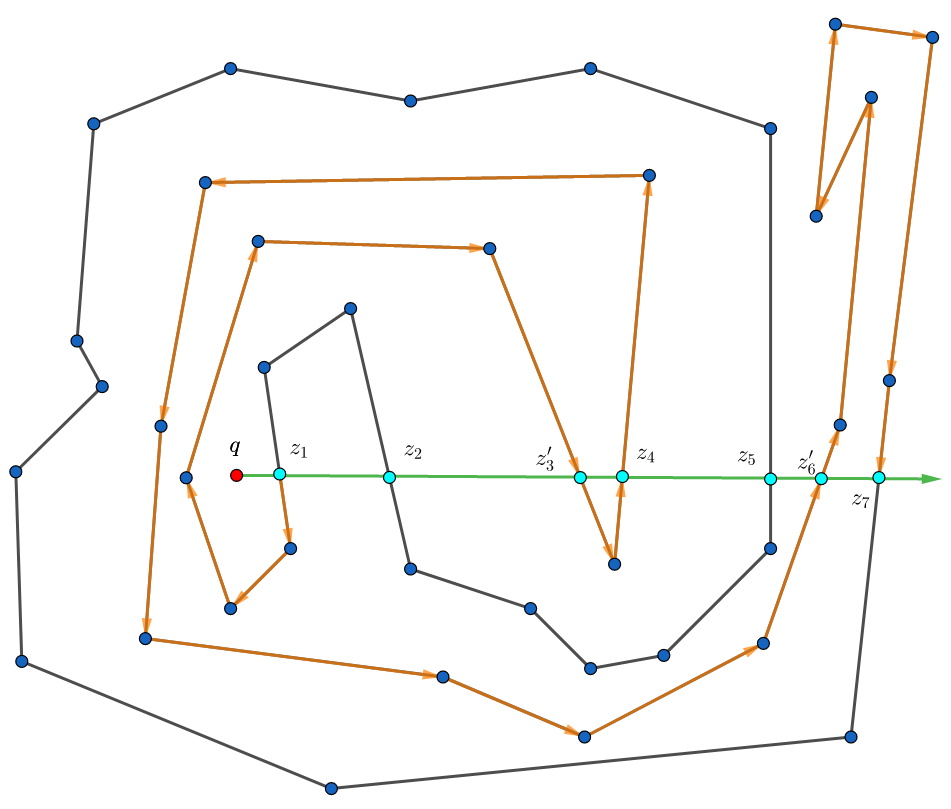
\includegraphics[width=0.45 \paperwidth]{images/Poda/9.png}
\end{frame}

\begin{frame}
  \centering 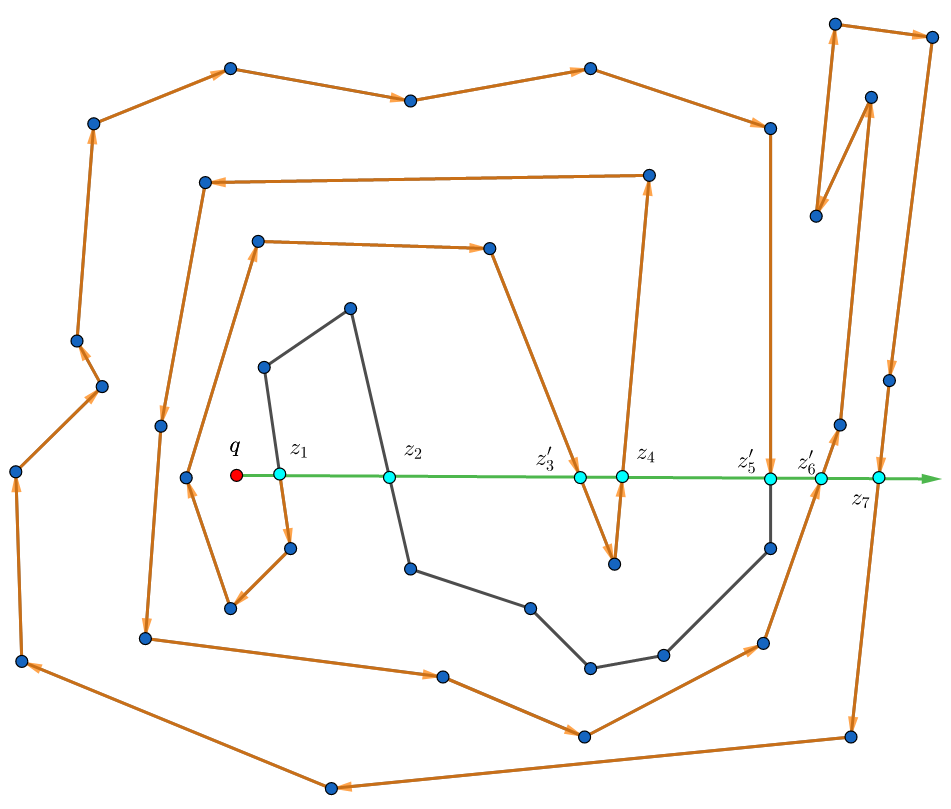
\includegraphics[width=0.45 \paperwidth]{images/Poda/10.png}
\end{frame}

\begin{frame}
  \centering 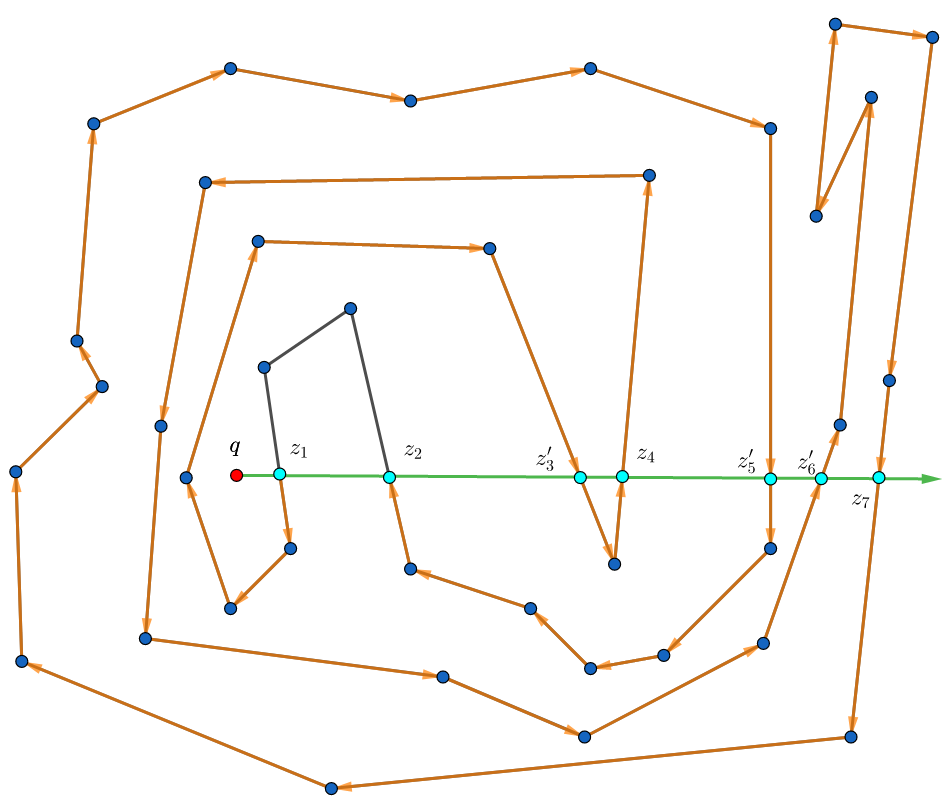
\includegraphics[width=0.45 \paperwidth]{images/Poda/11.png}
\end{frame}

\begin{frame}
  \centering 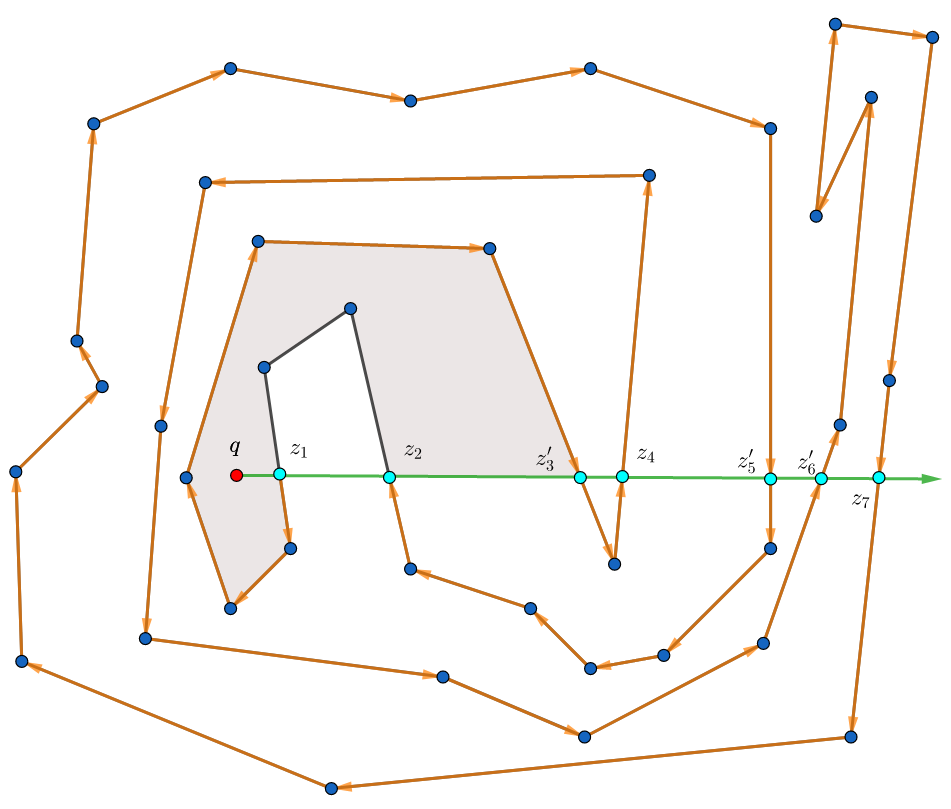
\includegraphics[width=0.45 \paperwidth]{images/Poda/12.png}
\end{frame}
\subsection{Análisis de complejidad.}

\begin{frame}
  \frametitle{Análisis de la complejidad.}
  \begin{enumerate}
  \item Lanzar el rayo lo hacemos en tiempo constante.
  \item Encontrar el primer punto que intersecta la frontera lo hacemos en $\mathcal{O}(\log n)$
    por medio de una búsqueda en las aristas de $P$.
  \item Clasificar las intersecciones lo hacemos en $\mathcal{O}(n)$, pues debemos recorrer el
    polígono $P$.
  \item Encontrar la primer arista respecto a $q$ tal que tenga sus dos extremos clasificados con
    diferente denominación $\{\text{abajo}, \text{ arriba}\}$ lo realizamos en $\mathcal{O}(n)$
    al recorrer nuevamente nuestro polígono.
  \end{enumerate}
\end{frame}
